\documentclass[12pt,letterpaper]{article}

% Evidencia: GA4-220501095-AA2-EV03
% Compilar con LaTeX Workshop o: latexmk -pdf GA4-220501095-AA2-EV03.tex
% El contenido usa caracteres ASCII para evitar problemas de codificacion.

\usepackage[spanish,es-nodecimaldot,shorthands=off]{babel}
\usepackage[T1]{fontenc}
\usepackage[utf8]{inputenc}
\usepackage{lmodern}
\usepackage{geometry}
\usepackage{setspace}
\usepackage{array}
\usepackage{longtable}
\usepackage{enumitem}
\usepackage{xcolor}
\usepackage{titlesec}
\usepackage{fancyhdr}
\usepackage{graphicx}
\usepackage{pdflscape}
\usepackage{hyperref}

% ==================== DATOS CONFIGURABLES ====================
\newcommand{\institucion}{Servicio Nacional de Aprendizaje -- SENA}
\newcommand{\programa}{Analisis y Desarrollo de Software}
\newcommand{\tituloTrabajo}{Bases conceptuales acerca del Lenguaje Unificado de Modelado y patrones de diseno}
\newcommand{\codigoEvidencia}{GA4-220501095-AA2-EV03}
\newcommand{\nombreProyecto}{Sistema de Gestion de Citas SAC}
\newcommand{\aprendiz}{Kevin Andres Granados Daza}
\newcommand{\instructor}{[Jesus Ramirez]}
\newcommand{\ficha}{[3389015]}
\newcommand{\ciudad}{Bogota D. C.}
\newcommand{\fechaEntrega}{[25 de septiembre de 2026]}
% ==============================================================

\geometry{top=2.54cm,bottom=2.54cm,left=2.54cm,right=2.54cm}
\onehalfspacing
\setlength{\parindent}{1.27cm}
\setlength{\parskip}{0pt}
\setlength{\headheight}{15pt}

\pagestyle{fancy}
\fancyhf{}
\fancyhead[L]{\codigoEvidencia}
\fancyhead[R]{\thepage}
\renewcommand{\headrulewidth}{0pt}

\titleformat{\section}{\normalfont\Large\bfseries\centering}{\thesection.}{0.5em}{}
\titleformat{\subsection}{\normalfont\large\bfseries}{\thesubsection.}{0.5em}{}

\begin{document}

\begin{titlepage}
    \centering
    \vspace*{2.5cm}
    {\Large \tituloTrabajo\par}
    \vspace{0.8cm}
    {\large Aplicacion al proyecto: \nombreProyecto\par}
    \vfill
    {\large \aprendiz\par}
    \vspace{1.5cm}
    {\large \institucion\par}
    {\large \programa\par}
    \vspace{1cm}
    {\large Evidencia: \codigoEvidencia\par}
    \vspace{1cm}
    {\large Instructor(a): \instructor\par}
    {\large Ficha: \ficha\par}
    \vfill
    {\large \ciudad\par}
    {\large \fechaEntrega\par}
\end{titlepage}

\section{Introduccion}

El desarrollo de software requiere herramientas que permitan comprender y comunicar de manera clara como funcionara un sistema antes de iniciar su construccion. Una de las herramientas mas utilizadas para este proposito es el Lenguaje Unificado de Modelado, conocido como UML por sus siglas en ingles. UML permite representar graficamente la estructura, los procesos, las interacciones y los cambios de estado de un sistema mediante diagramas estandarizados.

El uso de UML facilita la comunicacion entre analistas, desarrolladores, clientes y usuarios, ya que transforma necesidades expresadas en lenguaje natural en modelos visuales mas organizados. De esta manera se reducen ambiguedades, se identifican errores con anticipacion y se establecen bases claras para el diseno, la implementacion y las pruebas.

El presente informe desarrolla las bases conceptuales de UML, su importancia en el desarrollo de software, sus principales diagramas y su aplicacion al proyecto \nombreProyecto. Tambien se incluye un resumen elaborado en palabras propias y un glosario de terminologia esencial para comprender este lenguaje de modelado.

\section{Bases conceptuales del UML}

UML significa Unified Modeling Language o Lenguaje Unificado de Modelado. Es un lenguaje grafico utilizado para visualizar, especificar, construir y documentar los elementos de un sistema de software. Su objetivo no es reemplazar el codigo de programacion, sino representar de forma entendible como se organiza y como se comporta una solucion antes, durante y despues de su implementacion.

UML se utiliza principalmente en proyectos orientados a objetos porque permite representar clases, objetos, atributos, operaciones y relaciones. Sin embargo, tambien es util para analizar procesos de negocio, definir requisitos, documentar la arquitectura de una aplicacion y explicar la interaccion entre usuarios y componentes del sistema.

El termino unificado se relaciona con el hecho de que UML integra aportes de varias metodologias anteriores de modelado orientado a objetos. Con el tiempo se convirtio en un estandar ampliamente reconocido para documentar sistemas, debido a que ofrece una notacion comun que puede ser comprendida por diferentes integrantes de un equipo de desarrollo.

\subsection{Objetivos de UML}

Los principales objetivos de UML son los siguientes:

\begin{itemize}[leftmargin=1.2cm]
    \item Visualizar un sistema mediante modelos y diagramas.
    \item Especificar requisitos, estructuras, comportamientos e interacciones.
    \item Facilitar la comunicacion entre usuarios, clientes y equipo tecnico.
    \item Documentar las decisiones de analisis y diseno tomadas durante el proyecto.
    \item Identificar errores, dependencias y situaciones no consideradas antes de programar.
    \item Servir como guia para la construccion, prueba y mantenimiento del software.
    \item Mantener trazabilidad entre requisitos, procesos, clases y funcionalidades implementadas.
\end{itemize}

\subsection{UML no es un lenguaje de programacion}

Es importante diferenciar UML de un lenguaje de programacion. UML no se utiliza para ejecutar instrucciones directamente en un computador, como ocurre con Python, Java, JavaScript o C sharp. UML es un lenguaje de modelado: utiliza simbolos, lineas, figuras y reglas visuales para describir el sistema.

Por ejemplo, un diagrama de clases puede indicar que existe una clase llamada Cita con atributos como fecha y estado, y con metodos como confirmar() o cancelar(). Posteriormente, el programador utiliza esta informacion como referencia para implementar la clase en el lenguaje de programacion seleccionado.

\section{Importancia de UML en el desarrollo de software}

UML es importante porque permite analizar una solucion desde diferentes puntos de vista. Un solo diagrama no puede explicar todo un sistema; por esta razon UML ofrece diagramas para mostrar usuarios, requisitos, datos, procesos, mensajes, componentes y despliegue tecnico.

En las primeras etapas del proyecto, UML ayuda a comprender que necesita el usuario y cuales son las funciones esperadas. Durante el diseno, permite organizar las clases, los modulos y las relaciones entre componentes. En la implementacion, sirve como una guia para desarrollar el codigo. Finalmente, durante las pruebas y el mantenimiento, los diagramas ayudan a localizar los elementos que se deben verificar o modificar.

\begin{longtable}{|p{3.5cm}|p{5cm}|p{6.6cm}|}
\hline
\textbf{Etapa del proyecto} & \textbf{Aporte de UML} & \textbf{Ejemplo en el Sistema de Gestion de Citas SAC} \\
\hline
\endfirsthead
\hline
\textbf{Etapa del proyecto} & \textbf{Aporte de UML} & \textbf{Ejemplo en el Sistema de Gestion de Citas SAC} \\
\hline
\endhead
\hline
\endfoot
\hline
\endlastfoot

Levantamiento de requisitos & Permite identificar actores y funcionalidades esperadas. & Un diagrama de casos de uso muestra que Usuario puede agendar una cita y Administrador puede gestionar horarios. \\
\hline

Analisis & Permite estudiar procesos, reglas de negocio y escenarios alternativos. & Un diagrama de actividad representa que ocurre si el horario seleccionado ya no esta disponible. \\
\hline

Diseno & Permite definir clases, responsabilidades, relaciones y componentes. & Un diagrama de clases relaciona Usuario, Administrador, Cita, Horario y Notificacion. \\
\hline

Implementacion & Funciona como guia para construir el codigo y la base de datos. & La clase Cita se implementa con operaciones para crear, confirmar, cancelar y reprogramar. \\
\hline

Pruebas & Facilita crear escenarios de prueba a partir de requisitos y flujos. & Se prueba que una cita pendiente pueda confirmarse o rechazarse por un administrador. \\
\hline

Mantenimiento & Ayuda a comprender el sistema antes de corregir o ampliar funciones. & Un nuevo desarrollador puede consultar los diagramas para agregar recordatorios de citas. \\
\hline
\end{longtable}

\section{Clasificacion de diagramas UML}

Los diagramas UML se pueden agrupar en dos grandes categorias: diagramas estructurales y diagramas de comportamiento. Los primeros muestran las partes estaticas del sistema; los segundos representan lo que ocurre cuando los usuarios y objetos interactuan.

\subsection{Diagramas estructurales}

Los diagramas estructurales describen la organizacion interna del sistema. Permiten observar cuales elementos existen y como se relacionan entre si.

\begin{longtable}{|p{3.7cm}|p{5cm}|p{6.4cm}|}
\hline
\textbf{Diagrama} & \textbf{Que representa} & \textbf{Aplicacion al proyecto SAC} \\
\hline
\endfirsthead
\hline
\textbf{Diagrama} & \textbf{Que representa} & \textbf{Aplicacion al proyecto SAC} \\
\hline
\endhead
\hline
\endfoot
\hline
\endlastfoot

Diagrama de clases & Clases, atributos, operaciones y relaciones entre objetos. & Representa las clases Usuario, Administrador, Cita, Horario y Notificacion. \\
\hline

Diagrama de objetos & Instancias concretas de clases en un momento determinado. & Muestra un ejemplo especifico de un usuario con una cita asignada a un horario. \\
\hline

Diagrama de componentes & Modulos de software y sus dependencias. & Representa frontend, API REST, modulo de autenticacion, modulo de citas y base de datos. \\
\hline

Diagrama de despliegue & Nodos fisicos o virtuales donde se ejecuta el sistema. & Representa navegador, servidor web, servidor de aplicaciones y base de datos en la nube. \\
\hline

Diagrama de paquetes & Agrupacion logica de elementos relacionados. & Organiza paquetes como usuarios, citas, horarios, notificaciones y administracion. \\
\hline
\end{longtable}

\subsection{Diagramas de comportamiento}

Los diagramas de comportamiento describen acciones, procesos, decisiones y cambios que ocurren dentro del sistema.

\begin{longtable}{|p{3.7cm}|p{5cm}|p{6.4cm}|}
\hline
\textbf{Diagrama} & \textbf{Que representa} & \textbf{Aplicacion al proyecto SAC} \\
\hline
\endfirsthead
\hline
\textbf{Diagrama} & \textbf{Que representa} & \textbf{Aplicacion al proyecto SAC} \\
\hline
\endhead
\hline
\endfoot
\hline
\endlastfoot

Diagrama de casos de uso & Funcionalidades del sistema desde la perspectiva de actores externos. & Muestra que Usuario puede registrarse, iniciar sesion y agendar una cita; Administrador puede gestionar horarios y confirmar citas. \\
\hline

Diagrama de actividad & Flujo de acciones, decisiones y caminos alternativos de un proceso. & Describe los pasos para agendar una cita, validar disponibilidad y registrar la solicitud. \\
\hline

Diagrama de estados & Estados de un objeto y transiciones causadas por eventos. & Muestra los estados de una Cita: Pendiente, Confirmada, Rechazada, Cancelada, Reprogramada y Atendida. \\
\hline

Diagrama de secuencia & Orden temporal de los mensajes intercambiados entre participantes. & Representa como Usuario, interfaz, servicio de citas y base de datos participan en el agendamiento. \\
\hline

Diagrama de comunicacion & Relaciones y mensajes entre objetos, priorizando la estructura de colaboracion. & Muestra la colaboracion entre Usuario, Cita, Horario y Notificacion. \\
\hline
\end{longtable}

\section{Principales elementos de UML}

Los diagramas UML utilizan elementos visuales que tienen un significado definido. Aunque la forma cambia segun el tipo de diagrama, los elementos permiten representar participantes, datos, acciones, relaciones y restricciones.

\begin{itemize}[leftmargin=1.2cm]
    \item \textbf{Actor:} representa una persona, sistema externo u organizacion que interactua con el sistema.
    \item \textbf{Caso de uso:} representa una funcionalidad que genera valor para un actor.
    \item \textbf{Clase:} representa un tipo de objeto con atributos y operaciones comunes.
    \item \textbf{Objeto:} representa una instancia especifica de una clase.
    \item \textbf{Atributo:} representa una caracteristica o dato de una clase.
    \item \textbf{Operacion:} representa una accion o comportamiento que puede ejecutar una clase.
    \item \textbf{Asociacion:} representa una relacion entre clases.
    \item \textbf{Multiplicidad:} indica cuantas instancias pueden participar en una relacion, por ejemplo 1 a muchos.
    \item \textbf{Generalizacion:} representa herencia entre una clase general y otra especializada.
    \item \textbf{Dependencia:} indica que un elemento utiliza temporalmente a otro para realizar una tarea.
    \item \textbf{Interfaz:} define operaciones que una clase o componente debe ofrecer sin especificar todos sus detalles internos.
    \item \textbf{Mensaje:} comunicacion que un objeto envia a otro durante una interaccion.
    \item \textbf{Estado:} condicion en la que se encuentra un objeto en un momento determinado.
    \item \textbf{Transicion:} cambio de un estado a otro provocado por un evento o una condicion.
\end{itemize}

\section{Aplicacion de UML al Sistema de Gestion de Citas SAC}

El proyecto \nombreProyecto requiere diagramas UML para representar sus requisitos, estructura y comportamiento. Los modelos elaborados permiten relacionar las necesidades del usuario con el diseno orientado a objetos y con los procesos que se implementaran en la aplicacion web.

\subsection{Diagrama de casos de uso}

El diagrama de casos de uso permite identificar los actores principales y las acciones que cada uno puede realizar. Para el Sistema de Gestion de Citas SAC se reconocen dos actores principales: Usuario y Administrador.

El Usuario puede registrarse, iniciar sesion, consultar horarios, agendar una cita, cancelar una cita y reprogramar una cita. El Administrador puede gestionar horarios, visualizar las citas registradas, confirmar solicitudes, rechazar solicitudes y actualizar el estado de una cita.

% IMAGEN 1: Inserta aqui el diagrama de casos de uso generado en Draw.io.
% Guarda la imagen como: diagrama_casos_uso_sac.png
% Debe estar en la misma carpeta que este archivo .tex.
\begin{figure}[htbp]
    \centering
    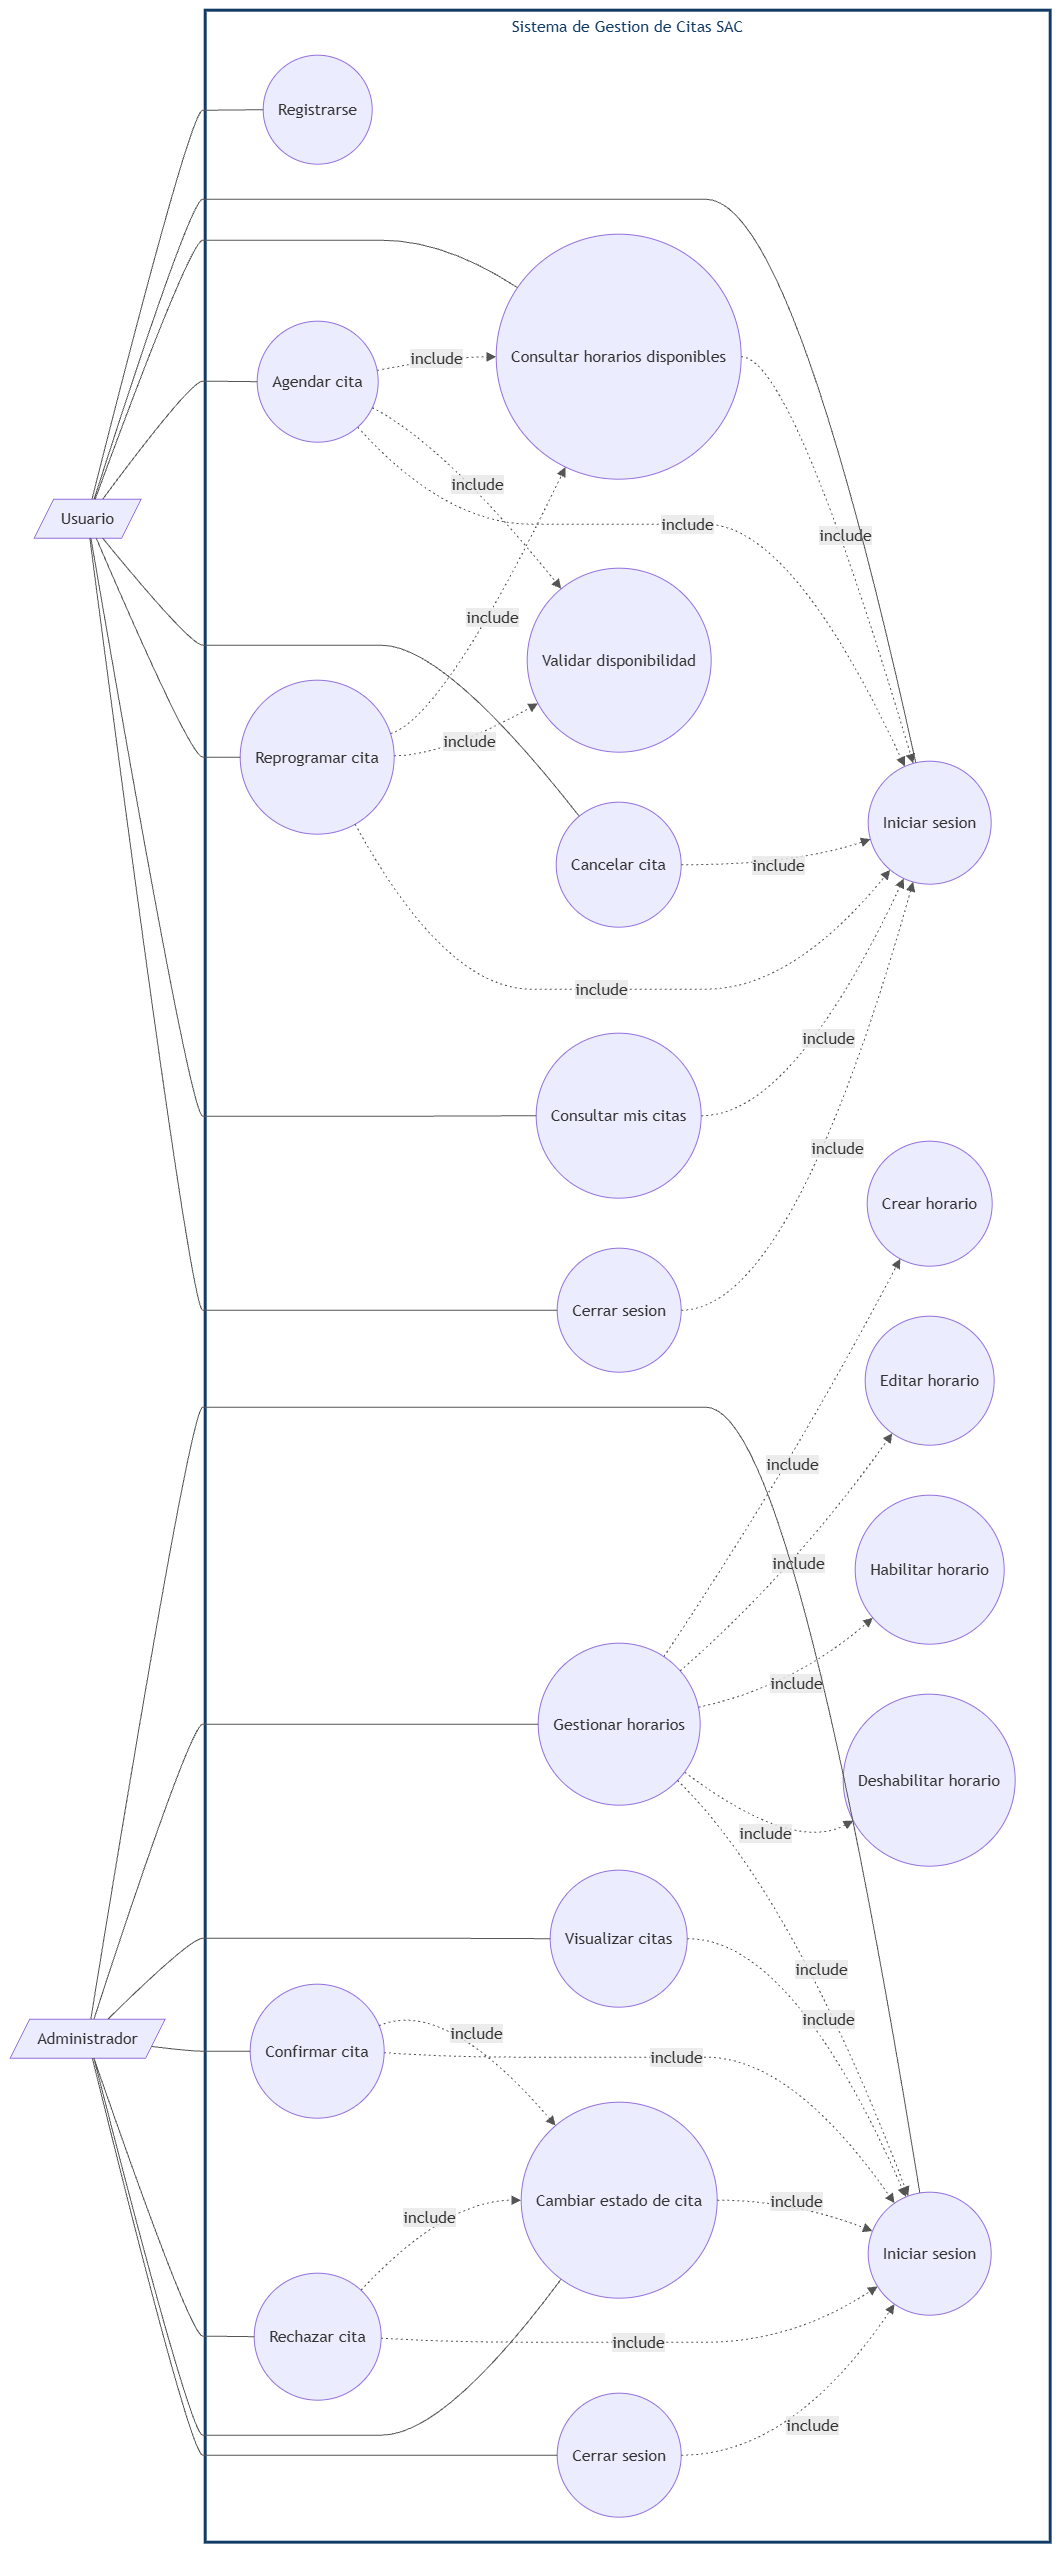
\includegraphics[width=0.5\textwidth]{Diagrama Casos.png}
    \caption{Diagrama de casos de uso del Sistema de Gestion de Citas SAC.}
    \label{fig:casos-uso-sac}
\end{figure}

Como se observa en la Figura~\ref{fig:casos-uso-sac}, cada funcionalidad parte de una necesidad concreta de los actores. Este diagrama permite delimitar el alcance funcional y sirve como base para elaborar casos de uso detallados, historias de usuario y pruebas funcionales.

\subsection{Diagrama de clases}

El diagrama de clases describe la estructura estatica del sistema y se relaciona directamente con la programacion orientada a objetos. Para este proyecto se proponen las clases Usuario, Administrador, Cita, Horario y Notificacion.

La clase Usuario representa a la persona que solicita y gestiona citas. La clase Administrador representa un usuario con permisos adicionales para gestionar horarios y solicitudes. La clase Cita registra la informacion de cada solicitud y su estado. La clase Horario representa una franja disponible para atencion, mientras que la clase Notificacion permite informar cambios importantes al usuario.

% IMAGEN 2: Opcional. Inserta aqui un diagrama de clases del SAC si lo generas en Draw.io.
% Guarda la imagen como: diagrama_clases_sac.png
% Si no vas a usar esta imagen, comenta o elimina todo el bloque figure.
%\begin{figure}[htbp]
%    \centering
%    \includegraphics[width=0.95\textwidth]{diagrama_clases_sac.png}
%    \caption{Diagrama de clases del Sistema de Gestion de Citas SAC.}
%    \label{fig:clases-sac}
%\end{figure}

La relacion entre Usuario y Administrador puede modelarse mediante herencia, ya que ambos comparten datos como nombre, correo y credenciales. Cita se relaciona con Usuario porque un usuario puede registrar varias citas. Cita tambien se asocia con Horario porque cada solicitud requiere un horario especifico. Esta estructura facilita aplicar abstraccion, encapsulamiento, herencia y polimorfismo durante la implementacion.

\subsection{Diagrama de actividad}

El diagrama de actividad permite representar los pasos necesarios para completar un proceso. En el caso del agendamiento de una cita, el usuario inicia sesion, consulta los horarios disponibles, selecciona uno, el sistema valida su disponibilidad y finalmente registra la cita con estado pendiente. Si el horario no esta disponible, el sistema solicita seleccionar otro.

% IMAGEN 3: Opcional. Inserta un diagrama de actividad del proceso Agendar Cita.
% Guarda la imagen como: diagrama_actividad_agendar_cita.png
%\begin{figure}[htbp]
%    \centering
%    \includegraphics[width=0.80\textwidth]{diagrama_actividad_agendar_cita.png}
%    \caption{Diagrama de actividad para el proceso de agendar una cita.}
%    \label{fig:actividad-agendar-cita}
%\end{figure}

Este tipo de diagrama es util para identificar decisiones, condiciones y flujos alternativos. Tambien ayuda a definir los casos de prueba necesarios para comprobar que el sistema responde adecuadamente ante diferentes situaciones.

\subsection{Diagrama de estados}

La clase Cita cambia de estado a medida que avanza el proceso de atencion. Un diagrama de estados permite representar estas transiciones y las acciones que las provocan.

Los estados principales propuestos para una cita son:

\begin{itemize}[leftmargin=1.2cm]
    \item Pendiente: la solicitud fue creada y espera revision o confirmacion.
    \item Confirmada: el administrador acepta la solicitud de cita.
    \item Rechazada: el administrador no acepta la solicitud.
    \item Cancelada: el usuario o administrador cancela una cita existente.
    \item Reprogramada: la cita cambia a un nuevo horario disponible.
    \item Atendida: la cita se realiza y el proceso termina.
\end{itemize}

% IMAGEN 4: Opcional. Inserta un diagrama de estados para Cita.
% Guarda la imagen como: diagrama_estados_cita.png
%\begin{figure}[htbp]
%    \centering
%    \includegraphics[width=0.85\textwidth]{diagrama_estados_cita.png}
%    \caption{Diagrama de estados de una cita en el Sistema de Gestion de Citas SAC.}
%    \label{fig:estados-cita}
%\end{figure}

\section{Patrones de diseno y su relacion con UML}

Los patrones de diseno son soluciones generales que pueden reutilizarse para resolver problemas frecuentes de organizacion y comunicacion entre objetos. No son fragmentos de codigo listos para copiar, sino estructuras o ideas que orientan la construccion de software flexible y mantenible.

UML es util para representar patrones de diseno porque los diagramas de clases y secuencia permiten visualizar las responsabilidades, interfaces y colaboraciones requeridas por cada patron. En un proyecto real, los patrones deben aplicarse solo cuando aporten una mejora clara y no como una obligacion innecesaria.

\begin{longtable}{|p{3.5cm}|p{4.6cm}|p{6.8cm}|}
\hline
\textbf{Patron} & \textbf{Proposito} & \textbf{Posible aplicacion en el SAC} \\
\hline
\endfirsthead
\hline
\textbf{Patron} & \textbf{Proposito} & \textbf{Posible aplicacion en el SAC} \\
\hline
\endhead
\hline
\endfoot
\hline
\endlastfoot

MVC & Separa el modelo de datos, la interfaz y el control de las solicitudes. & Permite separar las entidades Usuario, Cita y Horario de las vistas web y de los controladores que procesan las solicitudes. \\
\hline

Singleton & Garantiza una unica instancia controlada de una clase. & Puede utilizarse para centralizar la configuracion de conexion a base de datos cuando la arquitectura lo requiera. \\
\hline

Factory Method & Centraliza la creacion de objetos relacionados. & Puede crear diferentes tipos de notificacion, como confirmacion, cancelacion o reprogramacion. \\
\hline

Observer & Permite notificar a varios interesados cuando cambia el estado de un objeto. & Cuando una cita cambia de estado, se puede generar una notificacion para el usuario y el administrador. \\
\hline

Strategy & Permite intercambiar algoritmos o comportamientos sin modificar el objeto principal. & Puede utilizarse para cambiar el medio de envio de notificaciones entre correo, mensaje interno o SMS. \\
\hline
\end{longtable}

\section{Resumen de UML en palabras propias}

En mi concepto, UML es una forma de dibujar y organizar las ideas de un sistema antes de programarlo. Me permite entender quienes van a usar la aplicacion, que acciones pueden realizar y como se conectan los datos y procesos. No reemplaza el codigo, pero funciona como un plano que evita construir el software sin una direccion clara.

Considero que UML es importante porque cada diagrama muestra una parte distinta del proyecto. El diagrama de casos de uso ayuda a entender las necesidades de los usuarios; el diagrama de clases muestra como se organizan los objetos y sus responsabilidades; los diagramas de actividad explican los pasos de un proceso; y los diagramas de secuencia o estados ayudan a comprender el comportamiento del sistema en el tiempo.

En el Sistema de Gestion de Citas SAC, UML permite representar de manera ordenada como un usuario se registra, consulta horarios y solicita una cita, mientras que el administrador configura disponibilidad y confirma o rechaza solicitudes. Al tener estos modelos antes de programar, resulta mas facil detectar reglas importantes, como no permitir dos citas activas para el mismo horario o registrar los cambios de estado de cada cita.

En conclusion, UML ayuda a que el desarrollo de software sea mas claro, organizado y comunicable. Tambien facilita que el equipo pueda mantener y mejorar el sistema en el futuro, ya que los diagramas conservan una explicacion visual de las decisiones tomadas durante el proyecto.

\section{Glosario de terminologia UML}

\begin{longtable}{|p{3.8cm}|p{11.1cm}|}
\hline
\textbf{Termino} & \textbf{Explicacion en palabras propias} \\
\hline
\endfirsthead
\hline
\textbf{Termino} & \textbf{Explicacion en palabras propias} \\
\hline
\endhead
\hline
\endfoot
\hline
\endlastfoot

UML & Lenguaje grafico estandarizado que se utiliza para modelar, visualizar y documentar un sistema de software. \\
\hline

Modelo & Representacion simplificada de una parte del sistema real que permite comprenderlo antes de construirlo. \\
\hline

Diagrama & Representacion visual de elementos y relaciones de un sistema utilizando simbolos definidos por UML. \\
\hline

Actor & Persona, rol, organizacion o sistema externo que interactua con la aplicacion. \\
\hline

Caso de uso & Funcion o servicio que el sistema ofrece a un actor para satisfacer una necesidad. \\
\hline

Escenario & Ejemplo concreto de como se desarrolla un caso de uso, incluyendo pasos normales y situaciones alternativas. \\
\hline

Clase & Plantilla que define los datos y comportamientos comunes de un conjunto de objetos. \\
\hline

Objeto & Instancia concreta de una clase con valores propios en sus atributos. \\
\hline

Atributo & Dato que describe una caracteristica de una clase u objeto. \\
\hline

Operacion o metodo & Accion que una clase puede ejecutar para realizar una tarea o modificar su estado. \\
\hline

Asociacion & Relacion estructural que indica que dos clases se conocen o colaboran entre si. \\
\hline

Multiplicidad & Cantidad de objetos que pueden participar en una relacion, por ejemplo uno a uno o uno a muchos. \\
\hline

Agregacion & Relacion de todo y parte en la que las partes pueden existir independientemente del todo. \\
\hline

Composicion & Relacion fuerte de todo y parte en la que las partes dependen del ciclo de vida del objeto principal. \\
\hline

Generalizacion & Relacion que representa herencia entre una clase general y una clase mas especializada. \\
\hline

Dependencia & Relacion que indica que un elemento necesita utilizar temporalmente a otro para realizar una accion. \\
\hline

Interfaz & Contrato que define operaciones disponibles sin mostrar la implementacion interna. \\
\hline

Paquete & Elemento que agrupa clases, diagramas u otros componentes relacionados para organizar mejor el modelo. \\
\hline

Componente & Modulo reemplazable de software que proporciona una funcion especifica dentro de la aplicacion. \\
\hline

Nodo & Recurso fisico o virtual donde se despliega una parte del sistema, por ejemplo un servidor o dispositivo. \\
\hline

Mensaje & Comunicacion enviada de un objeto o participante a otro dentro de un diagrama de interaccion. \\
\hline

Linea de vida & Linea vertical de un participante en un diagrama de secuencia que muestra su existencia durante una interaccion. \\
\hline

Actividad & Paso o tarea que forma parte de un proceso o flujo de trabajo. \\
\hline

Decision & Punto de un diagrama de actividad donde el flujo toma caminos diferentes segun una condicion. \\
\hline

Estado & Situacion o condicion de un objeto en un momento determinado de su ciclo de vida. \\
\hline

Transicion & Cambio de un estado a otro causado por un evento, una accion o una condicion. \\
\hline

Evento & Suceso que puede producir una accion o un cambio de estado dentro del sistema. \\
\hline

Restriccion & Regla o condicion que limita como debe comportarse un elemento del modelo. \\
\hline

Estereotipo & Mecanismo de extension de UML que permite clasificar un elemento con un significado adicional, por ejemplo <<interface>>. \\
\hline
\end{longtable}

\section{Conclusiones}

UML es una herramienta fundamental para analizar y documentar sistemas de software porque permite representar visualmente sus requisitos, estructura y comportamiento. Su uso facilita que los diferentes participantes del proyecto compartan una misma comprension del sistema antes de iniciar la construccion del codigo.

Los diagramas estructurales y de comportamiento cumplen funciones complementarias. Los diagramas de clases, componentes y despliegue permiten entender como esta organizado el sistema, mientras que los diagramas de casos de uso, actividad, secuencia y estados permiten comprender que acciones se realizan y como cambia el sistema ante diferentes eventos.

La aplicacion de UML al Sistema de Gestion de Citas SAC permite organizar las funcionalidades de usuarios y administradores, definir las relaciones entre clases como Usuario, Cita y Horario, y representar los procesos de agendamiento, confirmacion, cancelacion y reprogramacion. Esto contribuye a que el diseno sea coherente con los requisitos definidos para el proyecto.

Finalmente, los patrones de diseno complementan UML al ofrecer soluciones reutilizables para estructurar el software. Aplicados de manera adecuada, ayudan a construir una aplicacion mas organizada, flexible y facil de mantener. Por esta razon, UML y los patrones de diseno son herramientas valiosas durante todo el ciclo de vida del desarrollo de software.

\end{document}
